\section{Debugging}
The diagram show qualitatively how much time is spent on fixing bugs (\%) versus development costs.
More than half the design cycle time is spent in the debug phase of the project.
(This data is fairly consistent across a number of articles, although several outliers had the number as high as 80\%.)
Therefore, first priority has to prevent the introduction of bugs to the system.
Second priority has to find and fix the bugs in a early stage of the project.

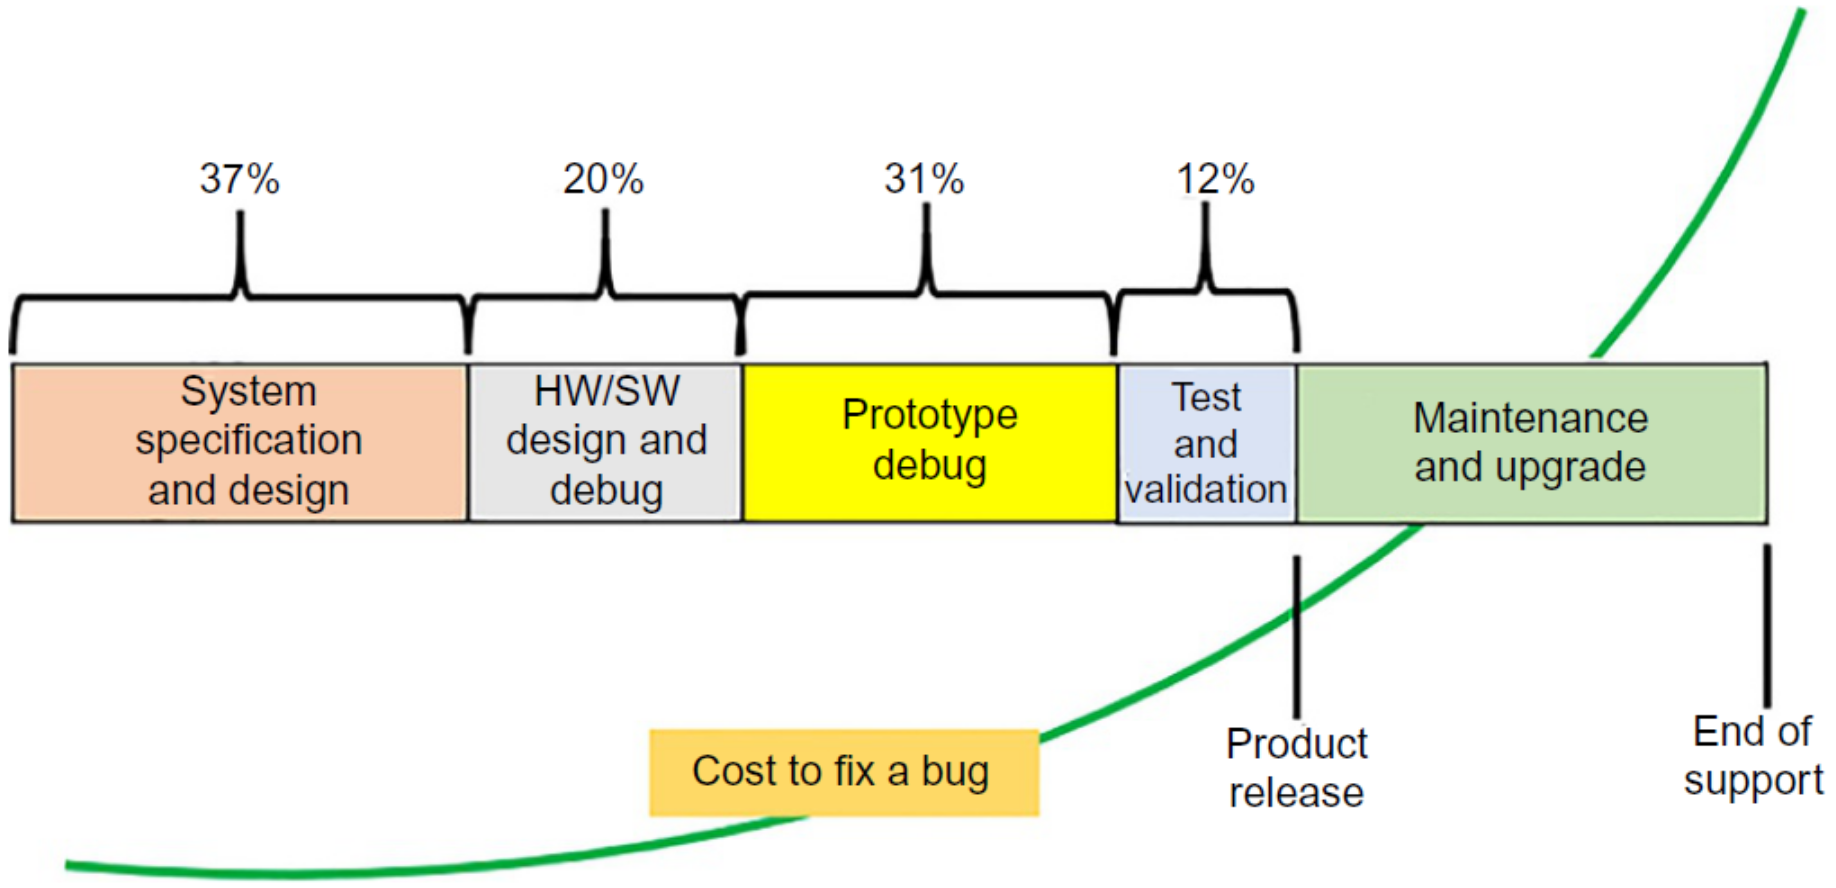
\includegraphics[width=0.6\textwidth]{images/Debugging/bugs_vs_cost}

\subsection{Prevention}
In the following points only a glimpse is given at certain topics to bug prevention:
\begin{itemize}
    \item Partition projects (small size of functions, modules, classes)
    \item Use Naming and style conventions
    \item Code defensive
          \begin{itemize}
              \item Never assume anything
              \item Use coding standards
              \item Keep your code as simple as possible because complexity breeds bugs.
          \end{itemize}
    \item Static Code analysis (Lint)
    \item Take compiler warnings seriously
    \item Test often
    \item Small repeatable test cases
    \item Continued integration test if possible
\end{itemize}

\subsection{Process}
\begin{itemize}
    \item Don't practice shotgun approach \glqq Try a bunch of changes at once and hope for the best\grqq
    \item Slow down
    \item Write down what you know
    \item Know your system
    \item Write down assumptions (hypothesis), investigation methods
    \item Explore the simple possibilities first
    \item Do differential testing
    \item Consider the solution best effort vs. price ratio
    \item Log the defect and the solution
\end{itemize}


\subsection{Profiling}
The profiling of tasks is the process to find out how the task behaves in manner of:
\begin{itemize}
    \item Performance load to the CPU
    \item Frequency
    \item Code coverage
    \item Memory usage
\end{itemize}
These are necessary values to determine if a system design is healthy or has potential risks.

\subsection{Tools}
There are many tools which help to debug embedded systems.
They differ:
\begin{itemize}
    \item In capability of online support with or without halting
    \item On influence on the embedded code and timing behaviour
    \item Availability during development process or release phase
    \item Pricing
\end{itemize}

\subsubsection{GPIOs}
Simplest and most cost effective tool are using GPIOs as debug information.
\begin{itemize}
    \item Toggling a PIN when entering an ISR and Leaving $\rightarrow$ Timing, frequency of ISR, Duration - ads execution time
    \item Toggling a PIN when in a certain Task and Leaving $\rightarrow$ Timing, frequency of Task, Duration - ads execution time
    \item Adding several PINs for states of the embedded system $\rightarrow$ overall status of the system (base for external logicanalyzer) - binds GPIOs
\end{itemize}

\subsubsection{Printf}
Simplest and often used in systems which can not be halted for debugging.
\begin{itemize}
    \item Sending a value in a task or ISR-timer $\rightarrow$ Value at a certain time or situation, + frequency is known - ads execution time
    \item Sending a value with timestamp $\rightarrow$ value / state at a certain time - ads execution time
\end{itemize}
$\Rightarrow$ A serial interface is needed: hardware or virtual (software)

\subsubsection{Trace}
More sophisticated approach.
Collecting data of a system: values / states with timestamp.
For offline analysis.
Searching for a certain situation and evaluating it.
The Collection can be achieved by using: GPIOs with logging, printf with logging, memory trace etc.

\subsubsection{Logic Analyzer}
Most sophisticated approach.
The logic analyzer uses the trace as source.
It is programmed with trigger rules.
Trigger rules can be very complex.
It reduces the effort to search in traces for a certain situation.
This help if the situation what is searched for is known.
Very good suited for verification testing after a bug fix.
Logic Analyzer are available as hardware solution with hardware probes, but also as software solution with software probes.

\subsection{STM32 Environment}
\subsubsection{ST-Link Virtual Serial Port (VCP)}
\columnratio{0.4}
\begin{paracol}{2}
    The ST-Links have a virtual serial port.
    This can be observed when connecting to a PC and checking the drivers.
    If the RX and TX Pis are connected to the MCU in the particular board (Nucleo, Discovery) can only be found out by investigating the boards manual.
    On our board nucleo STM32H745 it is the case… UART3 is connected to ST-Link.

    In tutorials you can find mostly the approach to replace the printf sub routines through a put or write routine.
    I would recommend not to replace the printf methods since it is used for other applications!

    Then you can use your favourite Console-Terminae: Putty, TerTerm…
    \switchcolumn
    \lstinputlisting[style=C, firstline=2]{snippets/Debugging/vcp.c}
\end{paracol}

\subsubsection{ST-Link Serial Wire Debug (SWD)}
Serial Wire Viewer adds:
\begin{itemize}
    \item Real time trace, that uses the SWD port and the SWO pin
    \item Advandced Debugging without halting the MCU
    \item Plots and logs
\end{itemize}

\subsubsection{ARM: Instrumental Trace Makrocell}
\begin{itemize}
    \item ITM is not the same as ETM (Embedded Trace Macrocell).
    \item ITM is an application driven trace that provides a high level software view.
    \item ITM enables tracing events and using instrumentations.
    \item Hardware triggers are used $\rightarrow$ fewer are available for breakpoints
\end{itemize}
Further information see: 63.6.3 Cortex-M7 instrumentation trace macrocell (ITM) technical reference Cortex-M7 ITM register map and reset values.
The ITM registers are located at address range 0xE0000000 to 0xE0000FFC, on the AHBD.

\begin{itemize}
    \item ITM periodically samples the program counter (PC)
    \item The debugger examinees the program counter to determine which function is being executed
\end{itemize}
$\rightarrow$ After running the application for a period of time you can determine which function are using most CPU cycles.
$\Rightarrow$ Profiling of software elements and tasks
